\documentclass[a4paper,10pt]{scrartcl}
\usepackage[utf8]{inputenc}
\usepackage[naustrian]{babel}
\usepackage{amsmath}
\usepackage{graphicx}
\usepackage{tabularx}
\usepackage{hyperref}

%opening
\title{Human Computer Interaction und Psychologie - Meilenstein 2}
\subtitle{Elektronisches Curriculum}
\author{Team 1 \\Pascal Attwenger, Philipp Hiermann, Sandra Markhart}

\begin{document}

\maketitle

\section*{Beschreibung der Prototypen}

\subsection*{Low-Fidelity-Prototyp}

Screenshots + Beschreibung

\subsection*{High-Fidelity-Prototyp}

\begin{description}
 \item[Url:] \url{http://wwwlab.cs.univie.ac.at/~a1151917/hci/}
 \item[Datei auf cewebs:]Meilenstein 2 - Team 1 - Webseite
  \begin{itemize}
  \item css/: CSS-Dateien von Bootstrap und eine angepasste CSS-Datei ``ecurriculum.css''
  \item js/: Java-Script-Dateien von Bootstrap
  \item fonts/: Fonts und Glyphicons von Bootstrap
  \item plan/: PHP-Dateien zum persönlichem Plan, der Überprüfung der aktuellen Session, Login/Logout und eine modifizierte csv-Datei
  \item ecurriculum/: PHP-Dateien zum eCurriculum
  \item img/: Logo der Universität Wien
 \end{itemize}
\end{description}

\begin{description}
 \item[Login-Daten:] 
 \begin{itemize}
  \item[]
  \item Matrikelnummer: a1234567
  \item Passwort: passwort
 \end{itemize}

\end{description}

\subsubsection*{Beschreibung und Funktionen}

\section*{Interview}

\subsection*{Vorgehensweise}

\subsection*{Ergebnisse}

\section*{Begründen der Designentscheidungen}
Nutzeranalyse aus Meilenstein 1

\section*{Typische Fehlermeldungen}

\subsubsection*{Aufrufen des persönlichen Plans ohne eingeloggt zu sein}

Eine typische Fehlermeldung ist, wenn der Benutzer den persönlichen Plan aufrufen will und sich noch nicht zuvor mit seinen Benutzerdaten eingeloggt hat,
da der persönliche Plan nur Studierenden zugänglich ist. Der Benutzer wird dann darauf hingewiesen, dass er sich einloggen muss.

\begin{quote}
 \textit{``Um auf Ihren persönlichen Plan zugreifen zu können, müssen Sie sich als Student mit Ihrer Matrikelnummer und Ihrem Passwort einloggen.''}
\end{quote} 

\begin{center}
 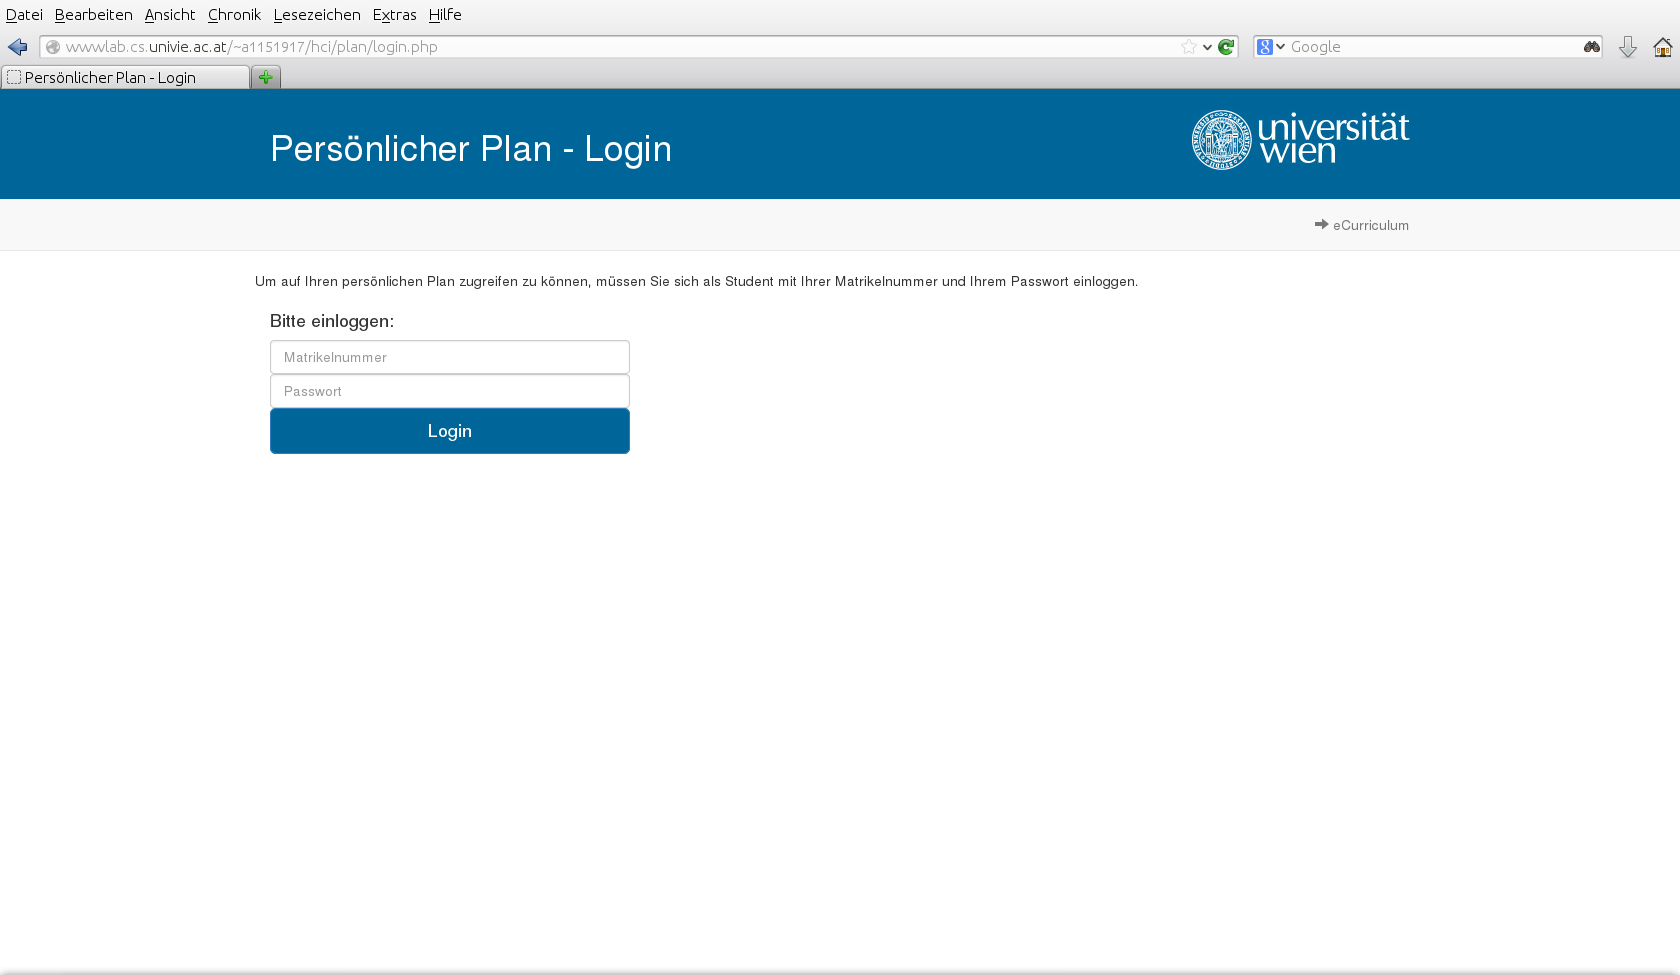
\includegraphics[scale=0.4]{./fehlermeldung1.png}
 % fehlermeldung1.png: 1680x975 pixel, 120dpi, 35.56x20.64 cm, bb=0 0 1008 585
\end{center}


\subsubsection*{Login mit falschem Benutzernamen oder falschem Passwort}

Eine weitere typische Fehlermeldung erscheint, wenn der Benutzer sich versucht einzuloggen, aber einen falschen Benutzernamen oder ein falsches Passwort eingibt.
Dieser wird dann je nachdem auf das falsche Passwort oder den falschen Benutzernamen hingewiesen.

\begin{quote}
 \textit{``Diese Matrikelnummer existiert nicht.''}
\end{quote} 

\begin{center}
 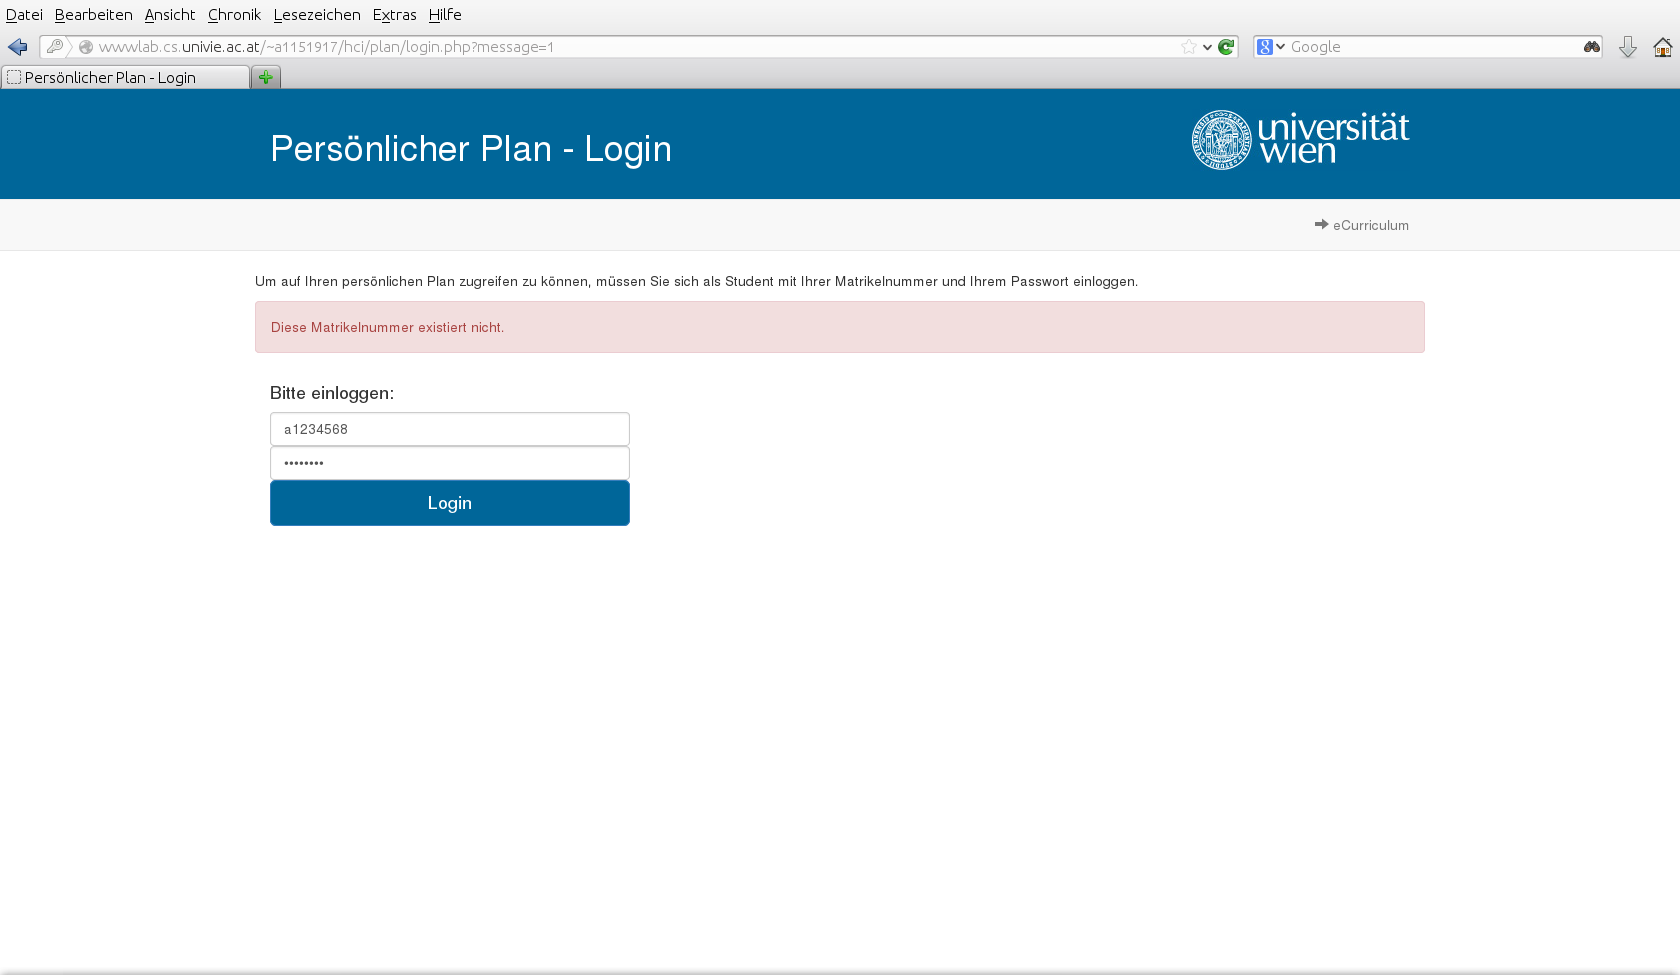
\includegraphics[scale=0.4]{./fehlermeldung2.png}
 % fehlermeldung1.png: 1680x975 pixel, 120dpi, 35.56x20.64 cm, bb=0 0 1008 585
\end{center}

Zusätzlich könnte zu der Fehlermeldung, dass die Matrikelnummer falsch ist dann noch die eingegebene Matrikelnummer angezeigt werden und gegebenenfalls darauf hingewiesen
werden, dass diese aus a + 7 Ziffern bestehen muss.

\begin{quote}
 \textit{``Das Passwort ist falsch.''}
\end{quote} 

\begin{center}
 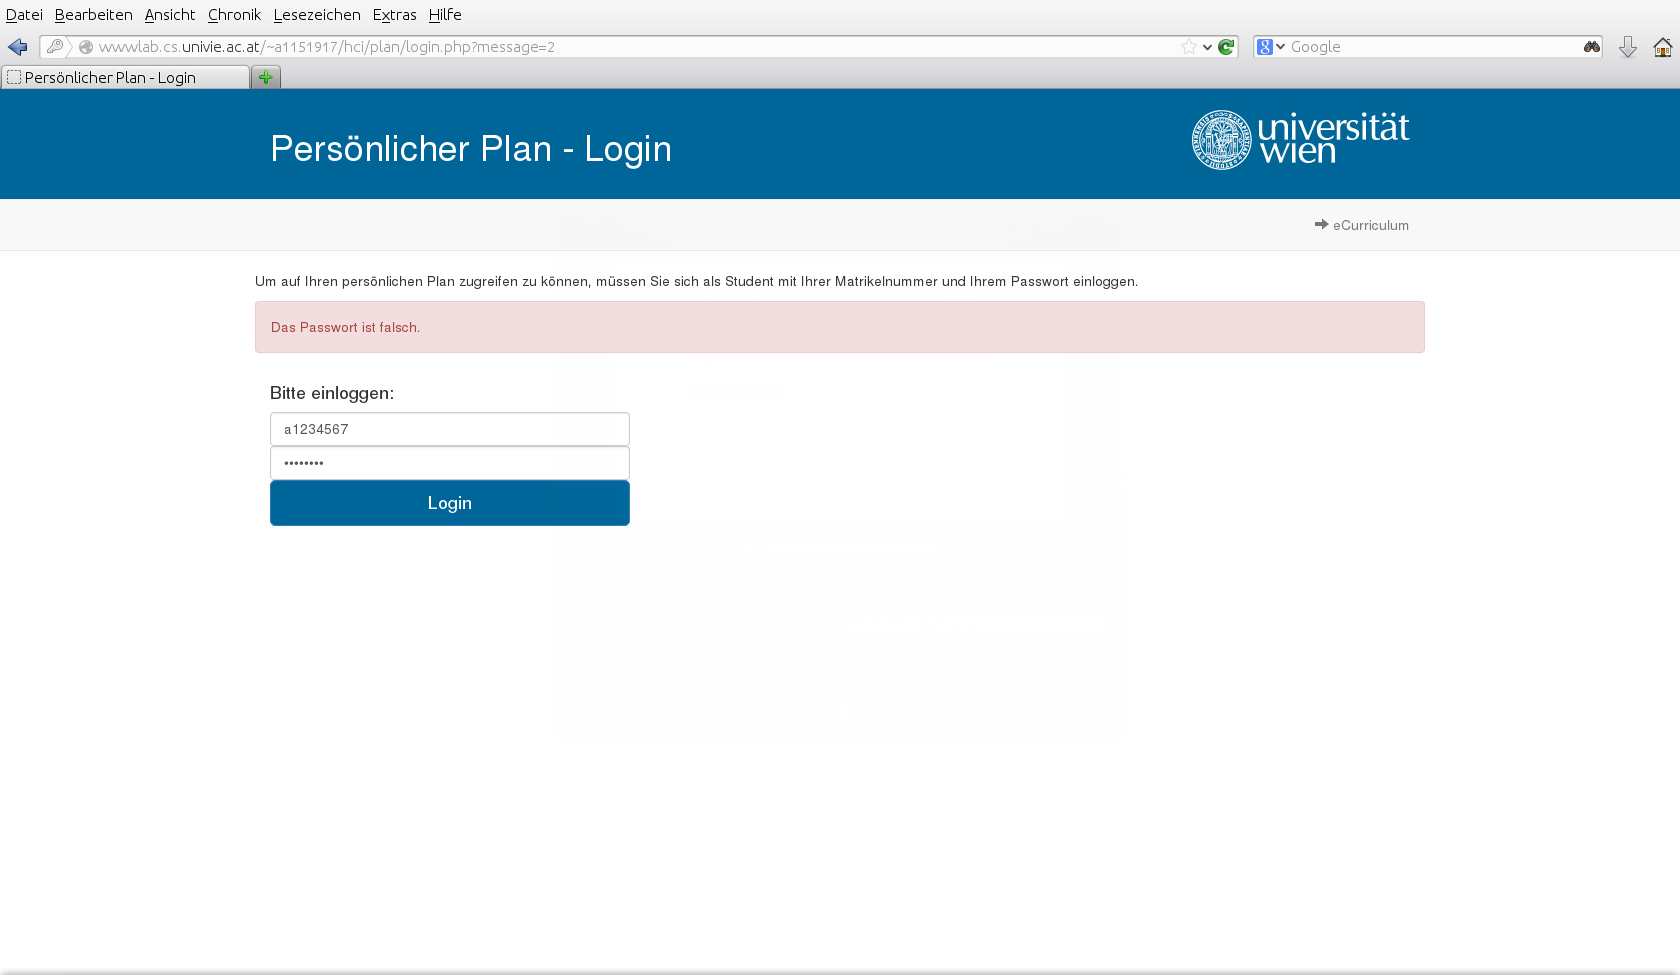
\includegraphics[scale=0.4]{./fehlermeldung3.png}
 % fehlermeldung1.png: 1680x975 pixel, 120dpi, 35.56x20.64 cm, bb=0 0 1008 585
\end{center}

Hier könnte zusätzlich entweder noch eine ``Passwort vergessen''-Funktion eingebaut werden, welche es ermöglicht das Passwort selbst zurückzusetzen oder einen
Hinweis auf z.B. den ZID gegeben werden, welcher in solchen Situationen weiterhilft.

\subsubsection*{Aufrufen eines nicht vorhandenen Moduls}

Auch könnte eine typische Fehlermeldung erscheinen, wenn eine Seite aufgerufen wird, welche nicht existiert. Dies kann hier auftreten wenn ein Modul aufgerufen wird, indem die Modulid in der Adressleiste
eingegeben wird, zu der kein Modul existiert.

\begin{quote}
 \textit{``Das Modul mit der Modulnummer 210324 existiert nicht.''}
\end{quote} 

\begin{center}
 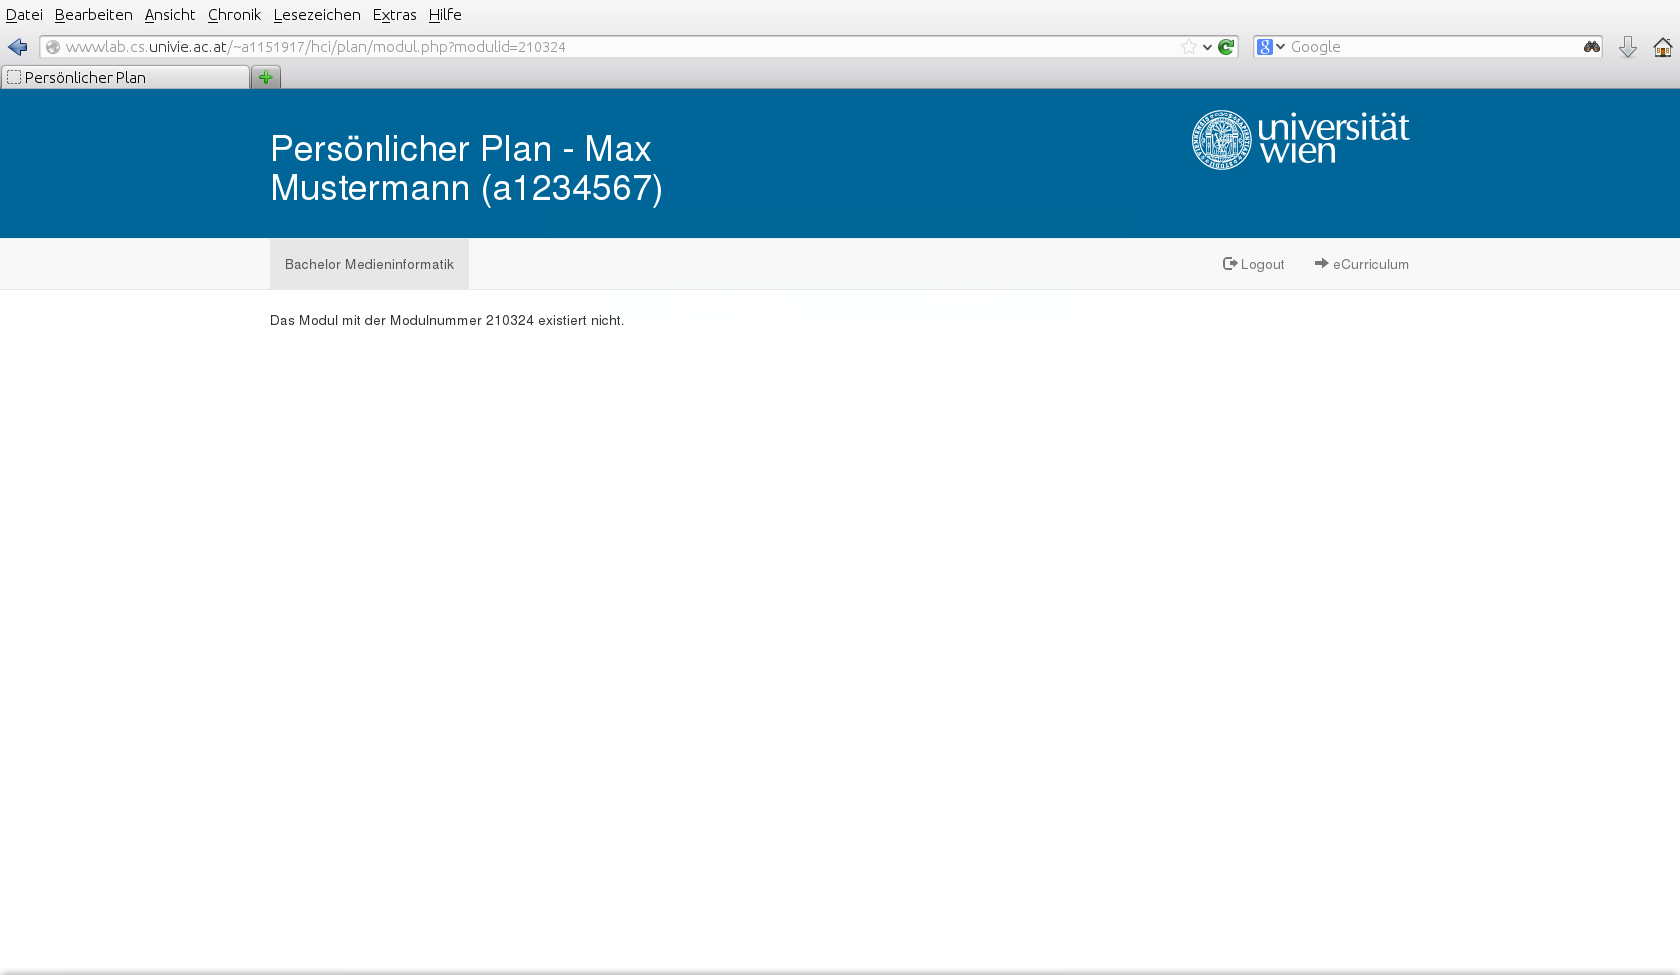
\includegraphics[scale=0.4]{./fehlermeldung4.png}
 % fehlermeldung1.png: 1680x975 pixel, 120dpi, 35.56x20.64 cm, bb=0 0 1008 585
\end{center}



\end{document}



